40. $\cfrac{x^2-4x+3}{2x-3}\leqslant\cfrac{x^2-4x+3}{x-2}\Leftrightarrow (x^2-4x+3)\left(\cfrac{1}{2x-3}-\cfrac{1}{x-2}\right)\leqslant0
\Leftrightarrow (x^2-4x+3)\cdot\cfrac{x-2-2x+3}{(2x-3)(x-2)}\leqslant0\Leftrightarrow\cfrac{-(x-3)(x-1)^2}{(2x-3)(x-2)}\leqslant0.$ Применив метод интервалов, найдём ответ: $x\in\{1\}\cup\left(\cfrac{3}{2};2\right)\cup[3;+\infty).$
\begin{figure}[ht!]
\center{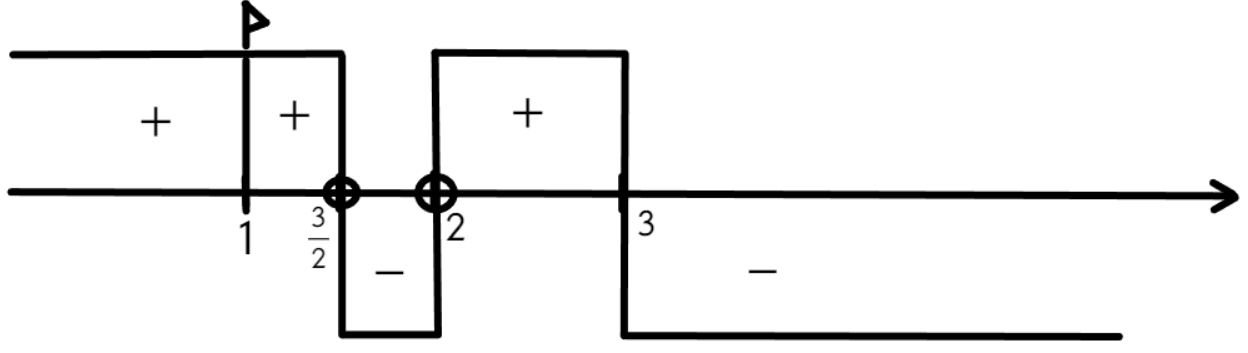
\includegraphics[scale=0.35]{ner9-40.png}}
\end{figure}\newpage\noindent
